\documentclass[tikz,border=9pt]{standalone}
\usepackage{amsmath}
\usepackage{pgfplots}
\pgfplotsset{compat=1.18}
\usetikzlibrary{arrows.meta}
\definecolor{ink}{HTML}{21352F}
\definecolor{teal}{HTML}{087F7B}
\definecolor{blue}{HTML}{4B77A8}
\definecolor{gold}{HTML}{C58B2A}
\definecolor{rose}{HTML}{B65A62}
\begin{document}
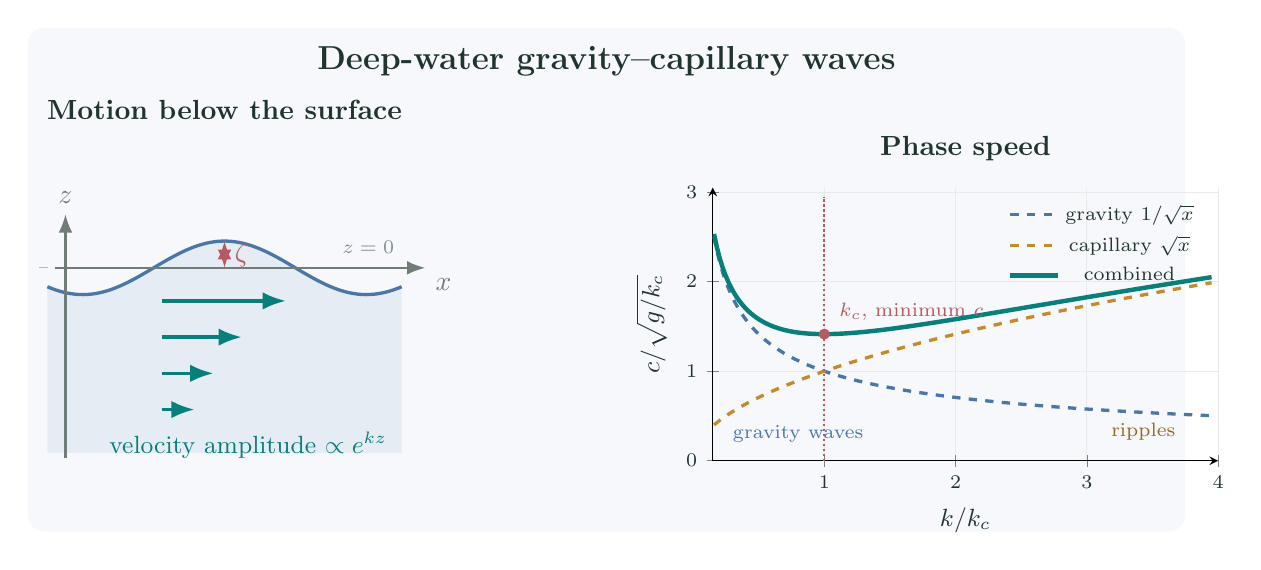
\begin{tikzpicture}[font=\sffamily,text=ink,>=Latex]
  \fill[blue!5,rounded corners=6pt] (-7.35,-3.15) rectangle (7.35,3.25);
  \node[font=\bfseries\large] at (0,2.82)
    {Deep-water gravity--capillary waves};

  \begin{scope}[shift={(-4.85,-.10)}]
    \node[font=\bfseries] at (0,2.30) {Motion below the surface};
    \path[fill=blue!14]
      plot[smooth,samples=90,domain=-2.25:2.25]
        (\x,{.30+.34*cos(100*\x)})
      --(2.25,-2.05)--(-2.25,-2.05)--cycle;
    \draw[blue,very thick,samples=90,domain=-2.25:2.25]
      plot (\x,{.30+.34*cos(100*\x)});
    \draw[ink!35,dashed] (-2.35,.30)--(2.35,.30);
    \node[ink!55,anchor=south east,font=\scriptsize]
      at (2.28,.36) {$z=0$};
    \draw[->,ink!65,thick] (-2.02,-2.12)--(-2.02,.98)
      node[above] {$z$};
    \draw[->,ink!65,thick] (-2.15,.30)--(2.55,.30)
      node[below right] {$x$};
    \draw[<->,rose,thick] (0,.30)--(0,.64)
      node[midway,right] {$\zeta$};

    \foreach \yy/\ll in {-.12/1.58,-.58/1.02,-1.04/.66,-1.50/.42} {
      \draw[teal,very thick,->] (-.80,\yy)--++(\ll,0);
    }
    \node[teal,align=center,font=\small] at (.30,-1.95)
      {velocity amplitude $\propto e^{kz}$};
  \end{scope}

  \begin{scope}[shift={(1.35,-2.25)}]
    \begin{axis}[
      width=8.0cm,height=5.05cm,
      title={Phase speed},
      title style={font=\bfseries},
      axis lines=left,
      xmin=.15,xmax=4.0,ymin=0,ymax=3.05,
      xlabel={$k/k_c$},
      ylabel={$c/\sqrt{g/k_c}$},
      domain=.16:3.95,samples=180,
      legend style={draw=none,fill=none,font=\scriptsize,
        at={(.98,.98)},anchor=north east},
      ticklabel style={font=\scriptsize},
      label style={font=\small},
      grid=major,grid style={ink!10}]
      \addplot[blue,very thick,dashed] {1/sqrt(x)};
      \addlegendentry{gravity $1/\sqrt{x}$}
      \addplot[gold,very thick,dashed] {sqrt(x)};
      \addlegendentry{capillary $\sqrt{x}$}
      \addplot[teal,ultra thick] {sqrt(1/x+x)};
      \addlegendentry{combined}
      \draw[rose,thick,densely dotted]
        (axis cs:1,0)--(axis cs:1,2.95);
      \fill[rose] (axis cs:1,1.41421356) circle (2pt);
      \node[rose,anchor=south west,font=\scriptsize]
        at (axis cs:1.04,1.46) {$k_c$, minimum $c$};
      \node[blue,anchor=west,font=\scriptsize]
        at (axis cs:.23,.30) {gravity waves};
      \node[gold!75!black,anchor=east,font=\scriptsize]
        at (axis cs:3.75,.32) {ripples};
    \end{axis}
  \end{scope}
\end{tikzpicture}
\end{document}
